\documentclass{article}
\usepackage[utf8]{inputenc}
\usepackage[italian]{babel}
\usepackage{graphicx}
\usepackage{hyperref}
\usepackage{pgf-pie} % Pacchetto per grafici a torta
\usepackage{lscape} % Per pagine orizzontali
\usepackage{caption} % Per personalizzare le didascalie
\usepackage[a4paper, margin=2.5cm]{geometry}

\title{Deadline 1 – Needfinding}
\author{Mattia Colombo, Carmen Giaccotto, Alessia Franchetti-Rosada \\Federico Previtali, Manoueil Michael Halim Riad Hanna \\ Valentina Petrignano, Michele Arrigoni}
\date{14 Ottobre 2024}

\begin{document}

\maketitle

\section{Introduzione}

\subsection{Dominio di interesse e perché lo abbiamo scelto}

Il nostro team è composto da: Mattia Colombo, Carmen Giaccotto, Alessia Franchetti-Rosada, Federico Previtali, Manoueil Michael Halim Riad Hanna, Valentina Petrignano e Michele Arrigoni.
Il nome del gruppo, Designer For Culture, è stato scelto sin da subito in quanto la nostra missione consiste nell’esplorare e sviluppare soluzioni innovative che uniscano tecnologia e cultura, con l’obiettivo di rendere l’arte e il patrimonio culturale più accessibili e coinvolgenti e promuovere una cittadinanza più consapevole e partecipativa. Abbiamo deciso di concentrarci su un target giovane, composto da ragazzi fra i 16 e i 19 anni che frequentano licei o che hanno da poco iniziato l’università. Il nostro intento iniziale è quello di capire che tipo di rapporto hanno gli adolescenti con l’arte e la cultura, in particolare quella delle loro città di appartenenza e capire quali sono i lori bisogni e le loro richieste per rendere più interattiva e coinvolgente l’esperienza museale.

\subsection{Partecipanti}

I partecipanti sono stati selezionati tramite conoscenze personali, tramite l’uso di piattaforme social come LinkedIn oppure tramite i contatti lasciati all’interno del survey da alcuni utenti.
Gli adolescenti, in particolare, sono stati coinvolti per comprendere le loro esigenze e motivazioni riguardo alle esperienze museali.
Come esperti di dominio abbiamo intervistato persone che lavorano nei musei da anni e che hanno esperienza adatta per darci consigli su cosa andrebbe e su cosa non andrebbe modificato all’interno dei musei. Abbiamo inoltre intervistato i genitori degli utenti rappresentativi, per vedere se la loro visione fosse la stessa dei figli e se fossero in grado di darci ulteriori informazioni da un punto di vista esterno, ma vicino a quello dei ragazzi.\\

\textbf{Utenti rappresentativi}: ragazzi tra i 16 e 19 anni.
\begin{itemize}
\item Aurora: Femmina, 19 anni, studentessa universitaria.
\item 	Daniele: Maschio, 19 anni, studente universitario.
\item 	Marco: Maschio, 18 anni, studente del quinto anno di Liceo Scientifico.
\item 	Ludovica: Femmina, 16 anni, studentessa del terzo anno di Liceo Scientifico.
\end{itemize}

\textbf{Esperti di Dominio}: persone con esperienza nel settore museale.
\begin{itemize}
\item Camilla: femmina, Education Officer presso il Museo della Scienza e della Tecnologia di Milano.
\item Carlo: maschio, Presidente dell’ArcheoClub di Siracusa e membro del consiglio direttivo dell’Associazione Nazionale Guide Turistiche.
\end{itemize}

\textbf{Utenti Affini}: genitori degli utenti rappresentativi.
\begin{itemize}
\item Danila: femmina, madre di due ragazzi, rispettivamente di 15 e 18 anni.
\item 	Paolo: maschio, padre di Marco (18 anni).
\item 	Stefania: femmina, madre di Ludovica (16 anni).
\end{itemize}

\subsection{Luogo delle Interviste}

Sulla base delle disponibilità dei partecipanti le interviste sono state svolte principalmente a distanza tramite un piattaforma di video conferenze.

\subsection{Organizzazione dell'Intervista}
Le interviste sono state organizzate in modo da raccogliere informazioni nel modo più completo possibile, in particolare si sono fatte considerazioni specifiche per:

\begin{itemize}
    \item I \textbf{gestori museali}, sfruttando il punto di vista di chi vive a contatto diretto con la categoria che ci interessa coinvolgere nel progetto. Sono state fatte domande focalizzate ad indagare come gli adolescenti interagiscono con l'arte e i musei, le sfide da affrontare nel coinvolgerli e quali potrebbero essere le migliori strategie per farlo.
    \item Gli \textbf{adolescenti}, indagando su quali siano le loro attuali esperienze e interazioni con i musei, le loro preferenze e quali sono le barriere, gli ostacoli o le motivazioni che condizionano la loro esperienza.
    \item I \textbf{genitori degli utenti rappresentativi}, per confrontare le loro opinioni con quelle dei figli e ottenere ulteriori informazioni da una prospettiva esterna, ma comunque vicina a quella dei giovani.
\end{itemize}

\subsection{Ruolo dei Membri del Gruppo}

Tutti i membri hanno partecipato all'organizzazione e alla realizzazione delle interviste. Non vi sono stati ruoli fissi per tutte le interviste per permettere ai partecipanti di svolgere diversi ruoli.
Per la formulazione delle domande ci siamo divisi in tre gruppi, uno da tre e due da due, e ogni gruppo ha creato le domande per l'apposito gruppo di utenti (rappresentativi, esperti di dominio e figure estreme).
Durante le interviste Carmen, Valentina e Mattia hanno principalmente assunto il ruolo di intervistatori, mentre Michele e Federico quello di osservatori.
I dati ottenuti sono poi stati rielaborati da Alessia e Manuel che hanno estratto le informazioni principali da mettere nella presentazione.
Come anticipato i ruoli descritti sono quelli che le persone hanno assunto prevalentemente, ma è bene specificare che ogni partecipante del gruppo ha dato il suo contributo in ogni fase delle interviste, a partire dalla formulazione delle domande, fino alla stesura della presentazione e del paper.

\subsection{Materiale Usato}

Durante le interviste sono stati utilizzati:

\begin{itemize}
    \item Registratore audio (previo consenso dei partecipanti) per garantire l'accuratezza dei dati raccolti.
    \item Notebook per prendere appunti durante le interviste.
    \item Software di videoconferenza.
\end{itemize}

\section{Risultati delle Interviste}
Partendo dalle interviste raccolte, abbiamo individuato i bisogni degli adolescenti nel contesto museale. Questi bisogni emergono dalle esperienze, opinioni e suggerimenti condivisi dagli intervistati, sia dagli adolescenti stessi che dai professionisti del settore museale.

\subsection{Bisogni degli Utenti e Citazioni Chiave Rilasciate}
\begin{enumerate}
    \item \textbf{Necessità di esperienze interattive e coinvolgenti}
    \begin{itemize}
        \item Gli adolescenti hanno bisogno di un modo per interagire attivamente con il museo attraverso attività che includano interazione, manualità o utilizzo di tecnologie per stimolare il loro interesse.
        \item \textbf{Riferimenti:}
        \begin{itemize}
            \item \textbf{Camilla}: ``I laboratori che includono elementi di interazione, manualità o l'uso di tecnologie sono molto più stimolanti per loro.''
            \item \textbf{Aurora}: ``Alla mostra di Van Gogh c'era una sala immersiva... Era una parte più interattiva rispetto al resto del percorso.''
            \item \textbf{Ludovica}: ``Mi piacciono le installazioni interattive. Penso che i musei dovrebbero offrire più esperienze interattive, specialmente per i giovani.''
            \item \textbf{Marco}: ``Apprezzo i musei in cui il visitatore può fare qualcosa, quelli interattivi.''
        \end{itemize}
    \end{itemize}

    \item \textbf{Necessità di esperienze immersive}
    \begin{itemize}
        \item Gli adolescenti hanno bisogno di poter immergersi nell'esperienza museale attraverso installazioni interattive o esperienze digitali immersive.
        \item \textbf{Riferimenti:}
        \begin{itemize}
            \item \textbf{Camilla}: ``Il nostro programma \emph{Digital Aesthetics} offre installazioni di arte digitale, immersiva e interattiva. Queste esperienze sono molto apprezzate dai ragazzi.''
            \item \textbf{Aurora}: ``Alla Sagrada Familia potevi vedere da vicino dettagli non visibili a occhio nudo grazie alla tecnologia.''
            \item \textbf{Ludovica}: ``Installazioni interattive dove puoi entrare nelle opere.''
        \end{itemize}
    \end{itemize}

    \item \textbf{Necessità di esplorazione individuale}
    \begin{itemize}
        \item Gli adolescenti hanno bisogno di un modo per esplorare e scoprire i musei in autonomia, piuttosto che attraverso visite di gruppo tradizionali.
        \item \textbf{Riferimenti:}
        \begin{itemize}
            \item \textbf{Aurora}: ``Trovo un po' noiose le visite di gruppo. Sarebbe meglio focalizzarsi su aspetti che permettano a ciascuno di avere un'esperienza completa anche girando autonomamente.''
            \item \textbf{Ludovica}: ``Preferisco scoprire le cose da sola o con qualcuno che conosca bene l'argomento e che possa spiegarmelo in modo più dinamico.''
        \end{itemize}
    \end{itemize}

    \item \textbf{Necessità di spazi sociali all'interno del museo}
    \begin{itemize}
        \item Gli adolescenti hanno bisogno che i musei diventino spazi sociali dove poter incontrarsi, discutere d'arte e sentirsi parte di una comunità.
        \item \textbf{Riferimenti:}
        \begin{itemize}
            \item \textbf{Ludovica}: ``Mi piacerebbe che ci fossero spazi dove i ragazzi possono incontrarsi e parlare d'arte.''
        \end{itemize}
    \end{itemize}

    \item \textbf{Necessità di un uso appropriato della tecnologia}
    \begin{itemize}
        \item Gli adolescenti hanno bisogno che la tecnologia sia utilizzata in modo appropriato nei musei, migliorando l'esperienza senza essere eccessiva o fuori contesto.
        \item \textbf{Riferimenti:}
        \begin{itemize}
            \item \textbf{Daniele}: ``La tecnologia deve essere usata in contesti e modi appropriati. Non vorrei vedere i quadri di Van Gogh scorrere sotto i miei piedi su uno schermo OLED; mi sembrerebbe inutile.''
            \item \textbf{Ludovica}: ``Non mi piace molto usare il telefono mentre sono al museo, preferisco godermi l'esperienza dal vivo.''
        \end{itemize}
    \end{itemize}

    \item \textbf{Necessità di partecipare attivamente e creare}
    \begin{itemize}
        \item Gli adolescenti hanno bisogno di opportunità per partecipare attivamente e creare qualcosa all'interno del museo, come workshop o laboratori.
        \item \textbf{Riferimenti:}
        \begin{itemize}
            \item \textbf{Ludovica}: ``Una parte del museo potrebbe essere dedicata alla creazione, dove i visitatori possono partecipare e creare qualcosa.''
            \item \textbf{Camilla}: ``I laboratori che combinano tecnologia e manualità permettono ai ragazzi di apprendere attraverso il fare.''
        \end{itemize}
    \end{itemize}

    \item \textbf{Necessità di apprendere attraverso metodi coinvolgenti}
    \begin{itemize}
        \item Gli adolescenti hanno bisogno di modi coinvolgenti per apprendere sulle opere e sugli autori, ad esempio attraverso video o storytelling.
        \item \textbf{Riferimenti:}
        \begin{itemize}
            \item \textbf{Marco}: ``Quando ci sono video che raccontano l'opera o la vita dell'autore, magari recitati da attori, è una cosa che apprezzo molto.''
        \end{itemize}
    \end{itemize}

    \item \textbf{Necessità di promozione attraverso i social media}
    \begin{itemize}
        \item Gli adolescenti hanno bisogno che i musei utilizzino maggiormente i social media per promuovere le attività e coinvolgere i giovani.
        \item \textbf{Riferimenti:}
        \begin{itemize}
            \item \textbf{Stefania}: ``Penso che i social media siano il mezzo principale. I musei dovrebbero sfruttare di più piattaforme come Instagram e TikTok.''
            \item \textbf{Daniele}: Ha suggerito un sistema di recensioni e un'app dedicata.
        \end{itemize}
    \end{itemize}

\end{enumerate}

\section{Risultati del Survey}

Abbiamo distribuito un sondaggio per raccogliere dati preliminari sugli utenti, in particolare adolescenti e giovani adulti. I risultati ci hanno fornito un quadro utile delle loro esperienze con i musei e delle loro aspettative.

\subsection{Link al questionario}

Il questionario completo può essere consultato al seguente link: \url{https://bit.ly/4eu3ox7}

\subsection{Demografia dei Partecipanti}

Il sondaggio ha coinvolto principalmente partecipanti di età compresa tra i 16-19 anni e oltre i 20 anni, con una rappresentanza femminile predominante. La maggior parte dei partecipanti risiede in piccole città o paesi, sebbene ci siano stati anche rispondenti provenienti da aree urbane.

\subsection{Frequenza di Visita ai Musei}

Quando è stato chiesto quante volte avevano visitato un museo negli ultimi 12 mesi, la maggior parte dei partecipanti ha indicato tra le 3 e le 5 visite, con alcuni che hanno dichiarato di aver visitato musei più di 5 volte.

\subsection{Grafici a Torta per i Dati del Survey}

\begin{figure}[h]
    \centering
    \begin{tikzpicture}
        \pie[text=legend, radius=3, color={red!30, blue!30, green!30, yellow!30}]{
            40/16-19 anni,
            35/20-25 anni,
            25/Oltre 25 anni
        }
    \end{tikzpicture}
    \caption{Distribuzione dell'età dei partecipanti.}
\end{figure}

\begin{figure}[h]
    \centering
    \begin{tikzpicture}
        \pie[text=legend, radius=3, color={red!50, blue!50}]{
            60/3-5 visite,
            40/Più di 5 visite
        }
    \end{tikzpicture}
    \caption{Frequenza di visita ai musei negli ultimi 12 mesi.}
\end{figure}
\newpage

\subsection{Suggerimenti per il Miglioramento dell'Esperienza Museale}

\begin{enumerate}
    \item \textbf{Migliorare l'interattività e il coinvolgimento e integrare tecnologie immersive}
        \begin{itemize}
            \item \textit{Mancanza di contenuti interattivi}: Un numero significativo di partecipanti ha indicato la ``mancanza di contenuti interattivi o interessanti'' come una delle principali difficoltà nell'esperienza museale. Molti adolescenti hanno espresso il desiderio di partecipare ad attività interattive e giochi all'interno del museo, indicando che tali attività li invoglierebbero a visitare più spesso.
            \item \textit{Preferenze per esposizioni interattive}: Le ``esposizioni interattive'' sono state citate come uno dei motivi principali che attirano i giovani al museo.
            \item \textit{Interesse per VR e AR}
            \item \textit{Desiderio di tecnologie innovative}
        \end{itemize}

    \item \textbf{Facilitare l'esplorazione individuale}
        \begin{itemize}
            \item \textit{Preferenza per l'autonomia}: Molti giovani preferiscono approfondire le informazioni leggendo le descrizioni accanto alle opere o cercando informazioni autonomamente tramite smartphone.
            \item \textit{Interesse per app personalizzate}: C'è un desiderio di avere app che consentano di personalizzare il percorso di visita in base agli interessi individuali.
        \end{itemize}

    \item \textbf{Offrire alternative alle guide fisiche}
        \begin{itemize}
            \item \textit{Interesse per audioguide su smartphone}: Molti partecipanti sarebbero più propensi a utilizzare audioguide se accessibili direttamente dal proprio smartphone con le proprie cuffie.
            \item \textit{Preferenza per dispositivi personali}: C'è una tendenza a preferire l'utilizzo di dispositivi personali per accedere ai contenuti, evitando dispositivi condivisi.
        \end{itemize}
    
    \item \textbf{Creazione di spazi sociali all'interno del museo}
        \begin{itemize}
            \item \textit{Interesse per la connessione sociale}: Alcuni partecipanti sarebbero interessati a un'app che permetta di connettersi con persone con interessi simili durante la visita.
            \item \textit{Desiderio di competizione amichevole}: L'idea di sfide e competizioni con amici o altri visitatori è stata accolta positivamente da diversi adolescenti.
        \end{itemize}

    \item \textbf{Uso appropriato e mirato della tecnologia}
        \begin{itemize}
            \item \textit{Importanza della facilità d'uso}: La ``facilità di navigazione nell'app'' è stata indicata come un elemento importante.
            \item \textit{Evitare sovraccarico tecnologico}: Alcuni partecipanti preferiscono non utilizzare eccessivamente dispositivi personali per non distogliere l'attenzione dalle opere.
        \end{itemize}
        
    \item \textbf{Promozione della partecipazione attiva e creativa}
        \begin{itemize}
            \item \textit{Desiderio di attività pratiche}: Gli adolescenti hanno mostrato interesse per eventi, laboratori tematici e attività che permettano un coinvolgimento attivo.
            \item \textit{Interesse per giochi e sfide}: La partecipazione a cacce al tesoro interattive e giochi competitivi è vista come un modo per rendere la visita più divertente.
        \end{itemize}

    \item \textbf{Apprendimento attraverso metodi coinvolgenti}
        \begin{itemize}
            \item \textit{Preferenza per esperienze interattive}: Le esperienze con materiale audiovisivo e interattivo sono considerate coinvolgenti e stimolanti.
            \item \textit{Interesse per storytelling e curiosità}: Scoprire curiosità e informazioni nascoste sulle opere è un forte incentivo per i giovani visitatori.
        \end{itemize}

    \item \textbf{Promozione attraverso i social media e piattaforme digitali}
        \begin{itemize}
            \item \textit{Utilizzo dei social media}: I giovani suggeriscono di utilizzare piattaforme come Instagram e TikTok per promuovere mostre ed eventi.
            \item \textit{Collaborazioni con influencer}: Coinvolgere figure popolari potrebbe aumentare l'attrattiva dei musei per gli adolescenti.
        \end{itemize}

    \item \textbf{Offrire esperienze autentiche e personalizzate}
        \begin{itemize}
            \item \textit{Personalizzazione del percorso}: La possibilità di personalizzare il percorso di visita è stata apprezzata.
            \item \textit{Desiderio di autenticità}: I giovani vogliono vivere esperienze genuine, senza eccessive mediazioni tecnologiche.
        \end{itemize}

    \item \textbf{Integrazione di visite virtuali a siti antichi o non accessibili}
        \begin{itemize}
            \item \textit{Interesse per tecnologie immersive}: L'uso di VR e AR per esplorare siti storici ha suscitato interesse.
        \end{itemize}

    \item \textbf{Semplificazione dell'accesso e della fruizione dei servizi}
        \begin{itemize}
            \item \textit{Difficoltà con code e procedure}: Le code e le procedure complicate per ottenere biglietti e audioguide sono viste come ostacoli.
            \item \textit{Desiderio di servizi digitali efficienti}: La possibilità di acquistare biglietti e accedere ad audioguide tramite smartphone è altamente apprezzata.
        \end{itemize}

    \item \textbf{Collaborazione con il settore educativo}
        \begin{itemize}
            \item \textit{Integrazione scolastica}: Molti partecipanti vorrebbero che le visite ai musei fossero più integrate nel contesto scolastico.
            \item \textit{Valore educativo}: I giovani riconoscono il potenziale dei musei nell'arricchire la propria formazione e crescita personale.
        \end{itemize}

    \item \textbf{Creazione di contenuti accessibili e inclusivi}
        \begin{itemize}
            \item \textit{Diversi livelli di conoscenza}: C'è la necessità di fornire contenuti adatti sia a esperti che a neofiti.
            \item \textit{Accessibilità linguistica}: L'opzione di avere contenuti in diverse lingue è considerata importante da alcuni partecipanti.
        \end{itemize}
\end{enumerate}

\subsection{Disponibilità a Partecipare a Ulteriori Interviste}

Abbiamo anche chiesto ai partecipanti se fossero disposti a rispondere a ulteriori domande o a partecipare a interviste individuali. La maggior parte ha preferito non essere contattata, anche se alcuni hanno lasciato i loro contatti per un coinvolgimento futuro.
\newpage

\subsection{Logica del survey}
Le domande seguono una logica condizionale: in base alle risposte ottenute nella prima sezione, alcune domande nella seconda e terza sezione vengono omesse. Di seguito un'immagine che illustra la logica utilizzata.
\vspace*{\fill}
\begin{center}
    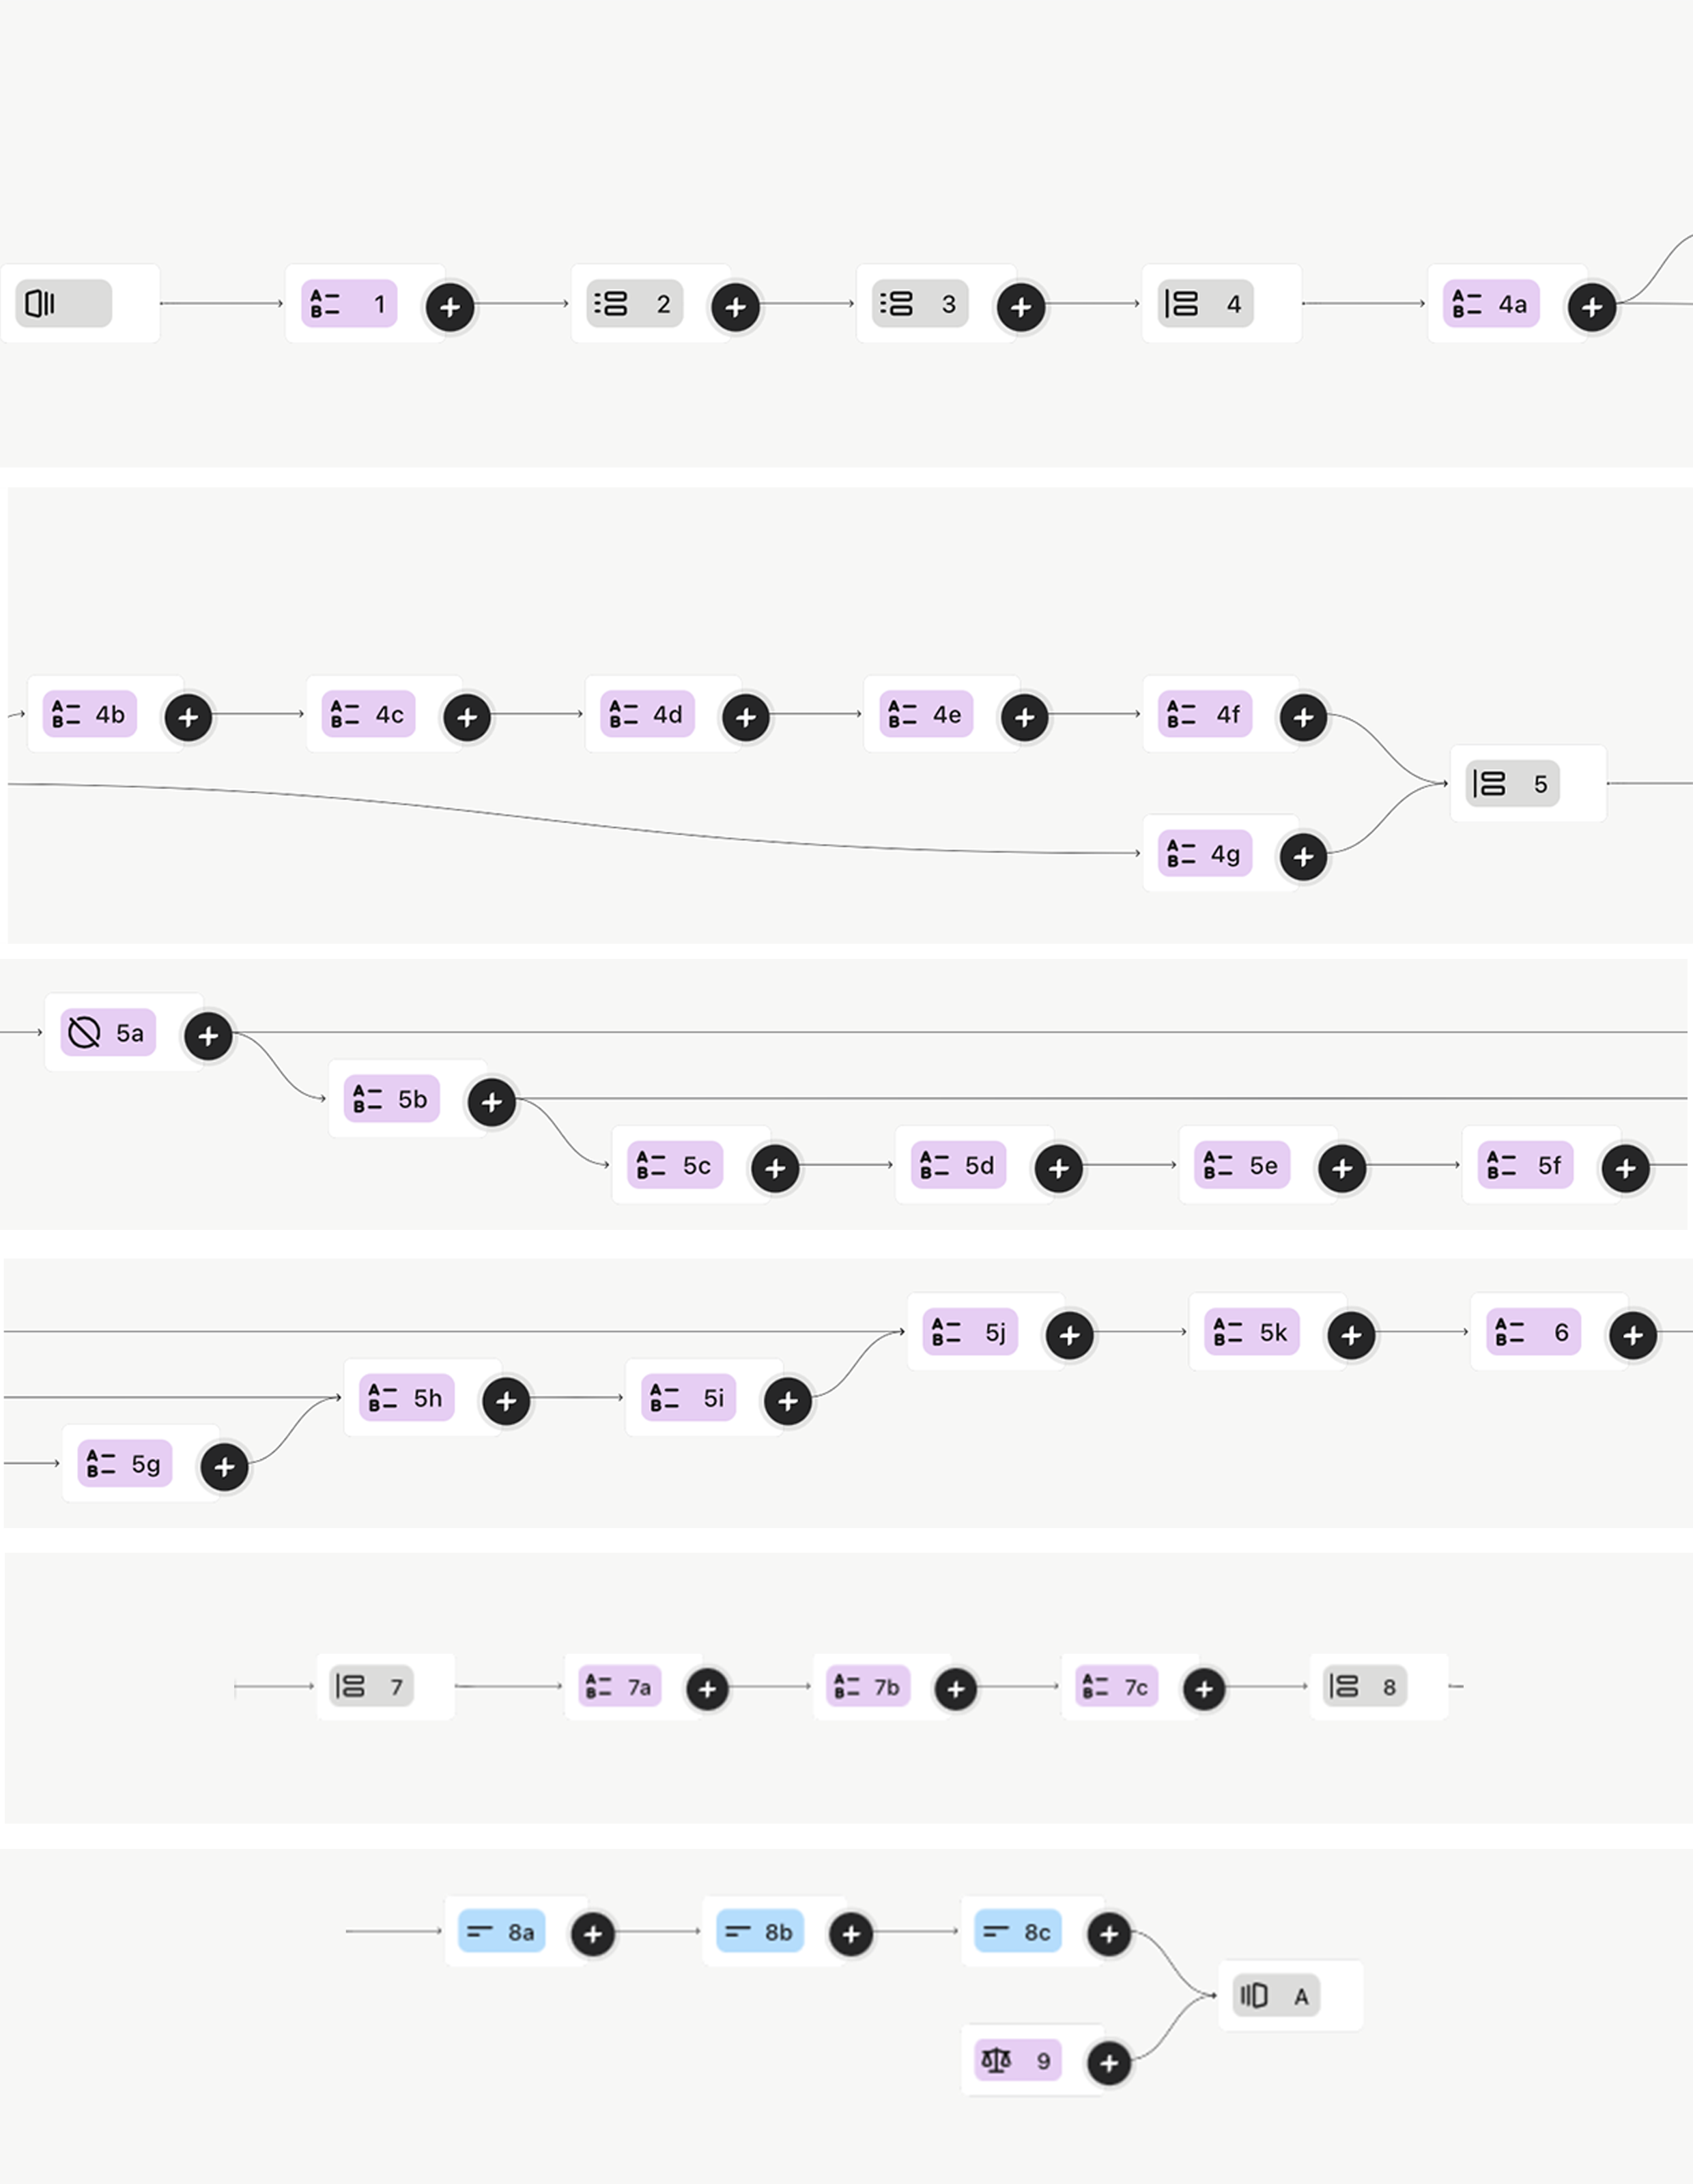
\includegraphics[width=\textwidth]{form_logic.png} % Immagine della logica del form (da inserire)
\end{center}
\vspace*{\fill}

\section{Foto Affinity Diagram Esercitazione}

\vspace*{\fill}
\begin{center}
    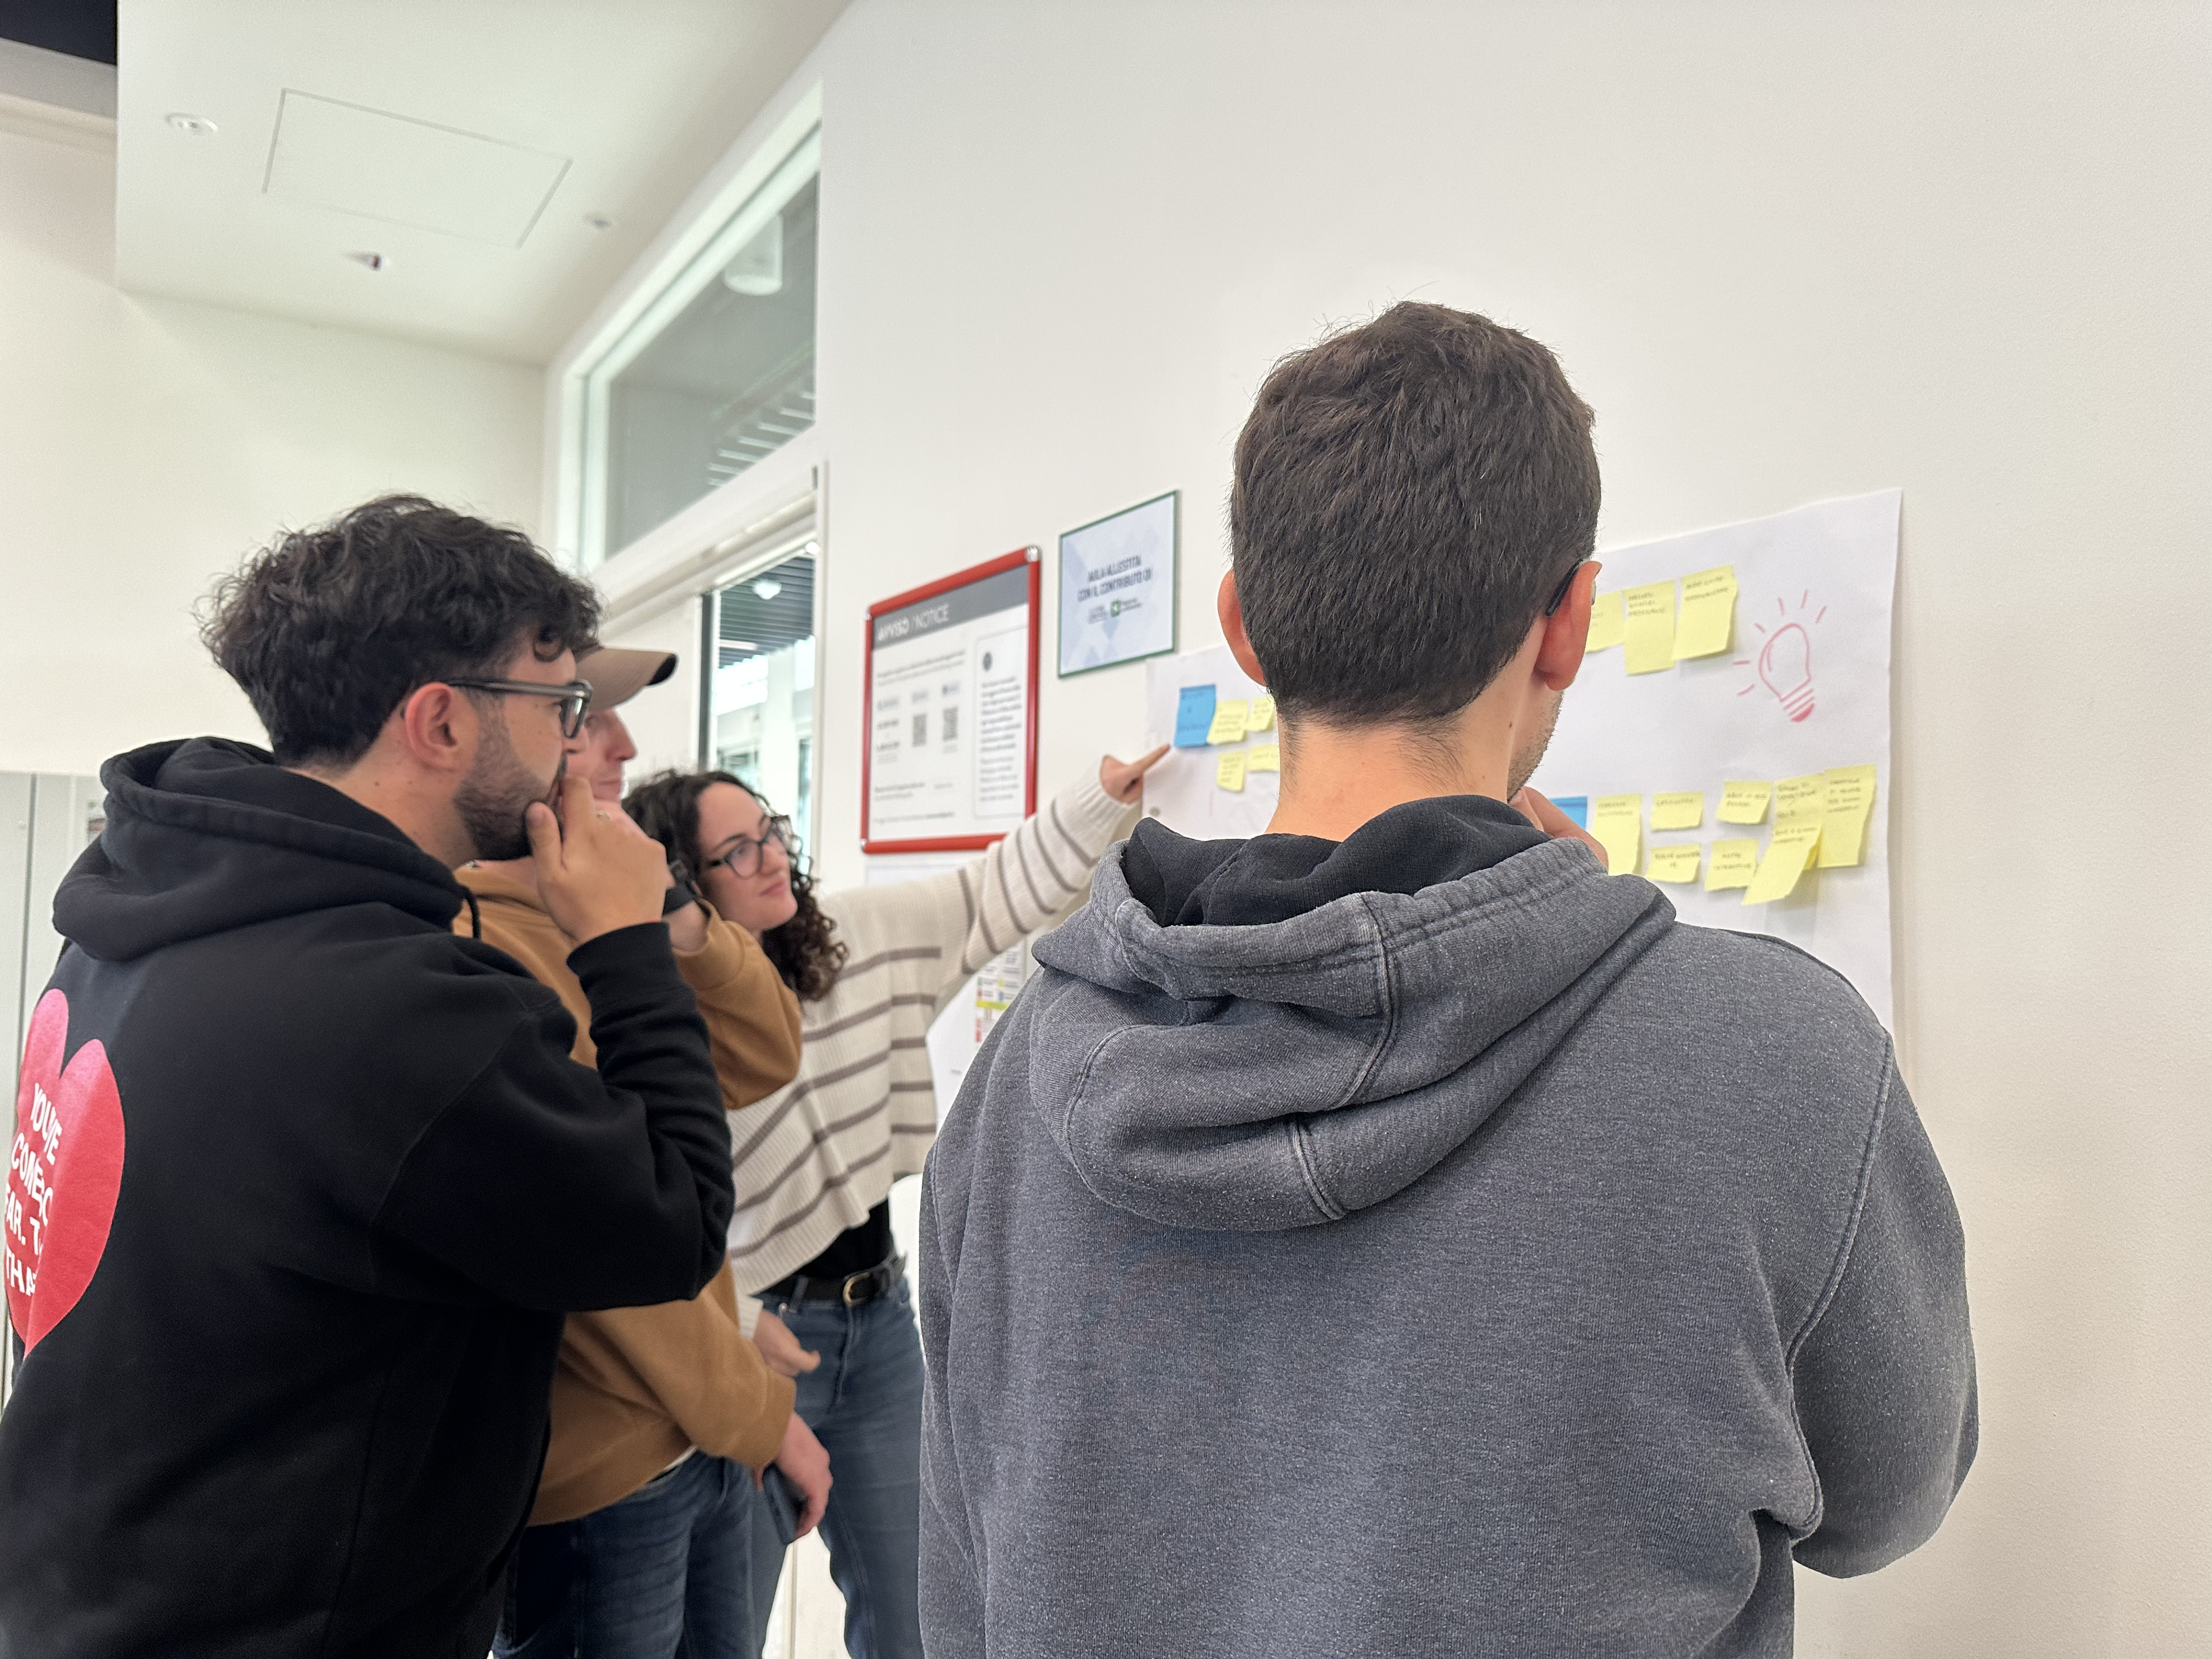
\includegraphics[width=\textwidth]{affinity_diagram.png} % Spazio per foto Affinity Diagram
\end{center}
\vspace*{\fill}

\section{Sintesi}

\subsection{Mappa Iniziale tra Utenti e Obiettivi}
\vspace*{\fill}
\begin{center}
    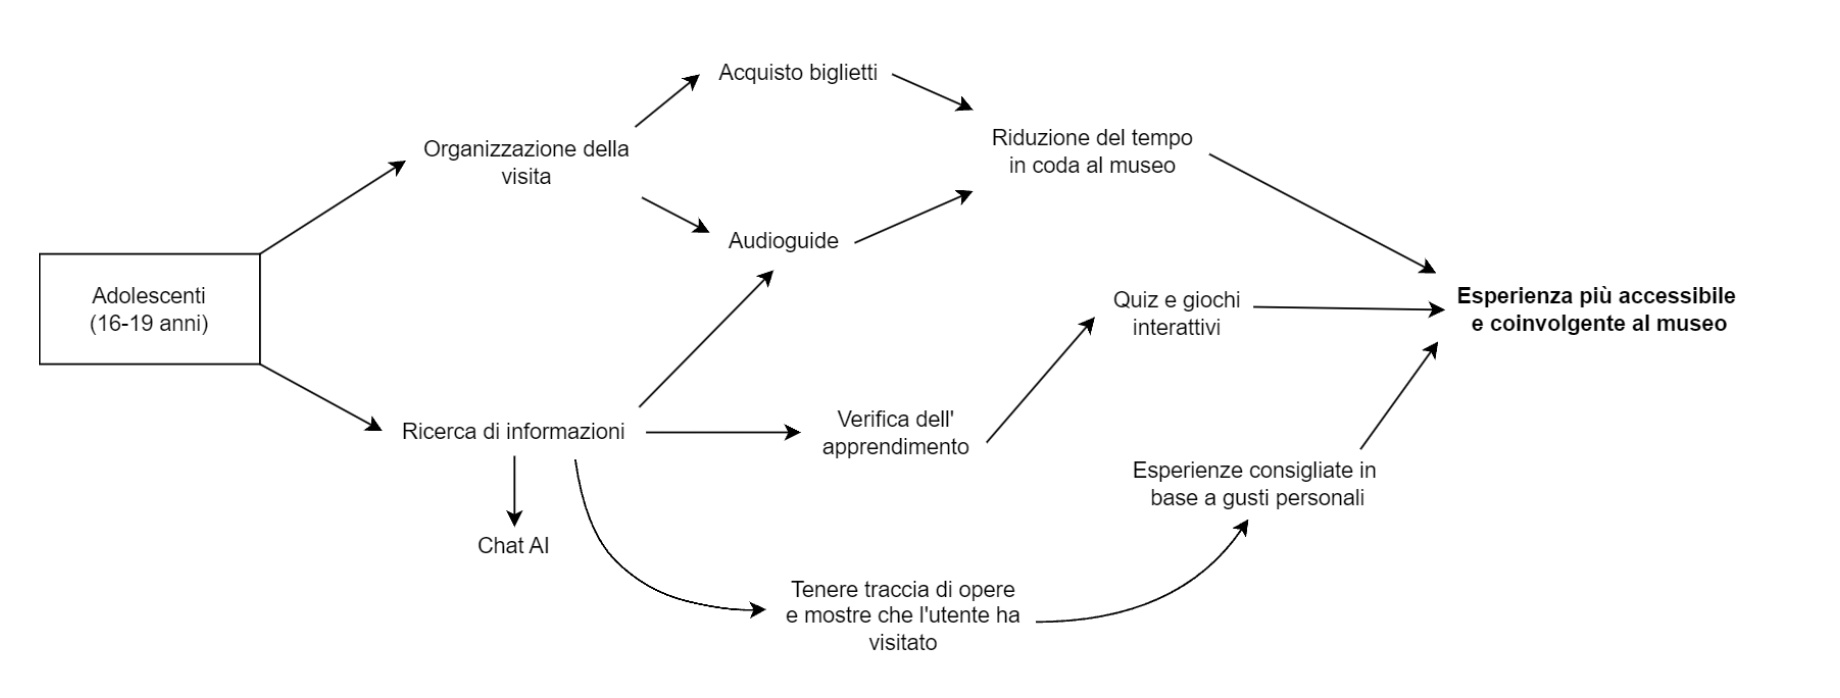
\includegraphics[width=\textwidth]{map.png}
\end{center}
\vspace*{\fill}

\section{Passi Futuri}

\begin{itemize}
    \item Analizzare ancora più in dettaglio i dati raccolti per identificare requisiti specifici.
    \item Sviluppare prototipi di soluzioni tecnologiche, interattive e coinvolgenti, basate sui bisogni emersi.
    \item Condurre test di usabilità con utenti rappresentativi per valutare le soluzioni proposte.
    \item Collaborare con musei e istituzioni per implementare e affinare le soluzioni.
\end{itemize}
\end{document}
